\textbf{PROBLEMA 1}
\vspace{20px}

Considere un disco metálico horizontal (A) de radio $a$ y de espesor despreciable tal y como se muestra en
la figura. El disco está conectado a un generador de tensión $V_0$. Para un punto P en el eje $z$ del disco y sobre
este,

\begin{center}
    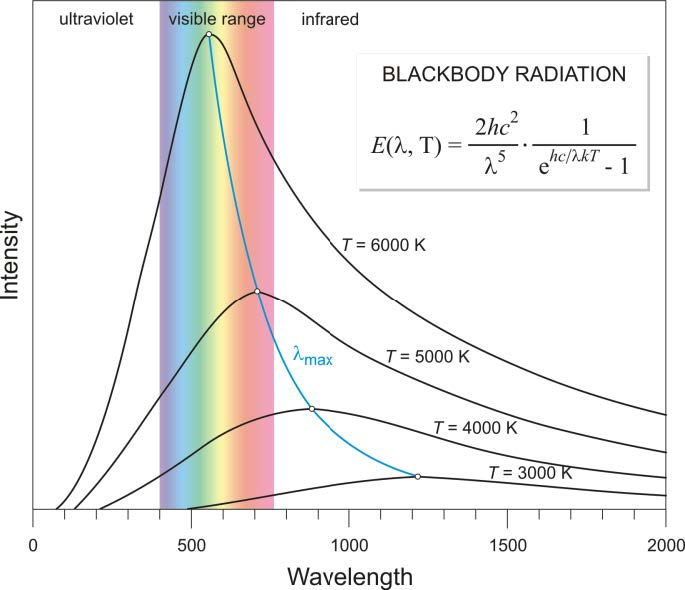
\includegraphics[width=6cm]{files/img1}
\end{center}

\begin{enumerate}[label=\alph*.]
    \item Calcule el potencial eléctrico a lo largo del eje $z$ y deduzca el valor de la densidad superficial de carga $\sigma$
    como función de $V_0$ y $a$. Ayuda: considere el disco como un conjunto infinito de anillos concéntricos.
    \item Calcule el campo eléctrico en un punto del eje $z$ sabiendo que $z > 0$.
    \item Suponga ahora que se coloca un segundo disco (B) de radio $b$ $(b \ll a)$, de espesor $e$ $(e \ll b)$ y densidad $\rho$
    de tal forma que el centro del disco (B) está prácticamente confundido con el origen. Este disco es libre
    de moverse en el eje $z$. Ambos discos están inicialmente en contacto eléctrico (de forma que la densidad
    superficial de carga es la misma en los dos discos). Determine el valor $V_s$ de la tensión umbral a partir la
    cual se produce el despegue del disco que está encima. Asuma que la aceleración de la gravedad es $g$.
\end{enumerate}

Ayuda. Utilice el siguiente resultado: $\int \frac{x}{\sqrt{a^2 + x^2}}\;dx = \sqrt {a^2 + x^2}$

\vspace{20px}
\textit{Solución:}
\\